Til at starte med, fremstalt vi nogle generelle samfundsmessige problemmer som vi står med ligenu, og de kan kategoriserer således:
\begin{itemize}
    \item Økonomi
    \item Miljø
    \item Klima
    \item Krig
\end{itemize}

Hvor vi underkategoriserede dem alt efter hvad der ligger i kategorierne

Økonomisk samfundsrelevanse problemer kan fx for høje priser, priserne på hvad kan man gør for at modkømpe pristigningerne, hvordan kan man forbedre og

\begin{figure}
    \centering
    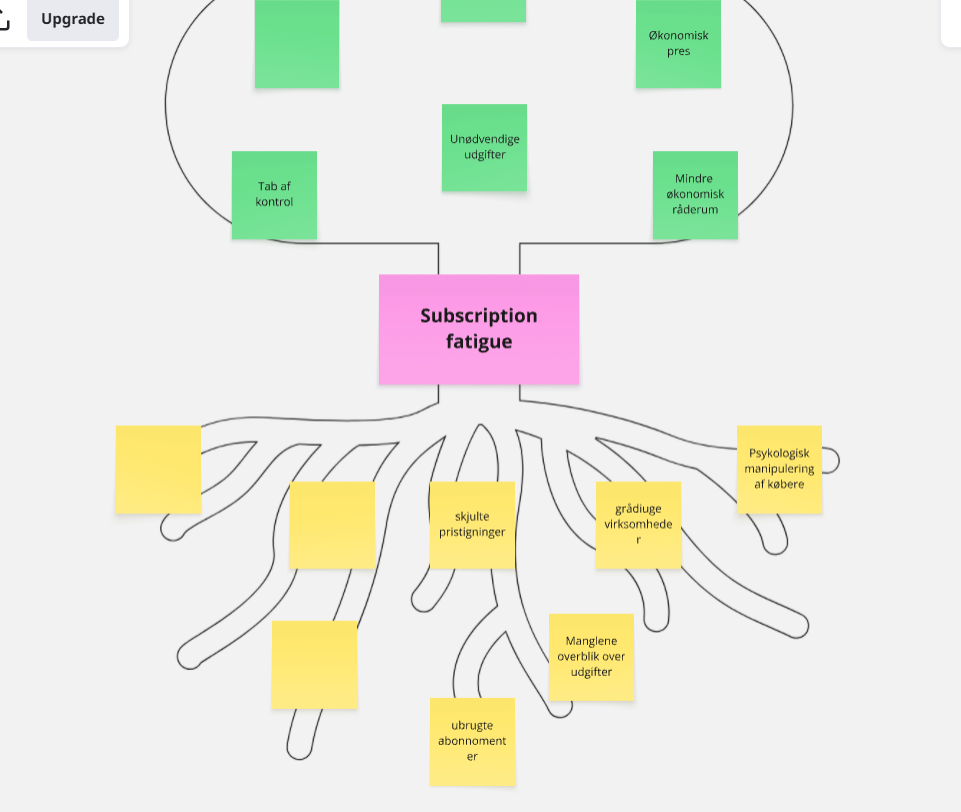
\includegraphics[width=\textwidth]{assets/problemtræ_udkast.png}
\end{figure}


Effektivisere den almene danskers privatøkonomi. 

således at vi kun kan ændre minimalt på en hverdag for en kæmpe forandeing i økonomien.


Miljømæssigt kan det være foruræning, affaldsortering og hvordan vi som samfund kan forbedre vores miljømæssige fodaftryk, med minimalt ændring.
Klima kan være hvordan vi kan mindske vores CO2 udslip, og hvordan vi kan forbedre vores klimaaftryk med minimalt ændring i hverdagen.
krig hvordan vi kan undgå tab af liv, eller forbedre våbende til et mindre dødeligt niveau, eller komme ud til de udsatte under en krig fx med feltrationer, uden at der nogle externe parter der skal riskiere sigselv.



En "dims", som kan se på din router hvilke hjemmesider/apps som bliver tilgået, og lave statestik over hvormeget hvilket bliver brugt, så vi herigennem kan lave statestik over hvilke subscriptions der bliver brugt mest, og hvilke der kan skæres fra, for at spare penge.


